
\section{The Cost of Identity Theft Calculated from ITS Data}
% \section{Methods}
\label{sec:comprehensive_cost_of_IDT}

\subsection{Modeling the Cost of Identity Theft}

To gain a clear picture of the real world impact of IDT, we developed a model to quantify its total cost. Our model calculates a comprehensive, per-victim cost for each survey year by monetizing the consequences of victimization across three categories: (1) direct financial and professional costs, (2) the opportunity cost of lost time, and (3) healthcare costs related to the incident. To ensure a valid cost comparison, all monetary values were adjusted to constant 2021 dollars using the annual average Consumer Price Index for All Urban Consumers (CPI-U) from the U.S. Bureau of Labor Statistics \cite{BLS_CPI, USInflationCalc_CPI}. For more information about the inflation adjustments, see Appendix \ref{app:inflation}.

\subsubsection{Category 1: Direct Financial and Professional Costs}
This category addresses the most immediate and explicit monetary losses that victims face. The primary component of this cost is the  direct/OOP loss that victims personally sustained and were not able to recover (i.e., stolen money not recovered). This excludes any fraudulent charges that were successfully disputed or covered by a financial institution, representing only the final realized financial harm to the victim. In addition to direct/OOP losses, this category also accounts for the cost of hiring professional legal services. While the ITS survey indicates whether a victim hired a lawyer or not, it does not record the amount paid. To monetize this expense, we assign an inflation adjusted cost of \$445 to each victim who reported hiring legal help. This fixed cost estimate is based on an average attorney hourly rate of around \$330, as reported in the 2023 Clio Legal Trends Report, and assumes approximately 1.5 hours of an attorney's time \cite{USNews_Lawyer}.

\subsubsection{Category 2: The Opportunity Cost of Lost Time}
Beyond direct financial loss, a significant cost comes from the time that victims sacrifice to resolve problems that arise from their IDT. This opportunity cost was quantified using the ``Hours Spent Resolving'' variable from the ITS dataset. To assign a monetary value to this lost time, the weighted average hours spent by victims each year was multiplied by the inflation adjusted average hourly wage for that corresponding year. The wage data was sourced from the U.S. Bureau of Labor Statistics' Current Employment Statistics Survey, which tracks average hourly earnings of all private nonfarm employees \cite{FRED_Wage}. This data was used because it represents the vast majority of the U.S. workforce and serves as a strong indicator of national wage trends. For more information regarding this data, see Appendix \ref{app:hourly_wages}.

\subsubsection{Category 3: Health and Well-being Costs}
While the significant emotional and psychological harm that victims suffer is difficult to quantify directly, our model addresses a measurable dimension of this distress by estimating the expenses related to seeking professional care. %To account for the measurable costs associated with the emotional and physical distress of victimization, our model also estimates the expenses related to seeking professional care.
Using responses from the ITS survey, we identified victims who reported visiting a medical professional, received counseling, or took medication due to distress related to the incident. Inflation adjusted cost estimates were then assigned based on national averages. Each medical visit was valued at \$133 \cite{DebtOrg_Doctor}, each therapy session at \$89 \cite{GoodRx_Therapy}, and a course of medication at \$54 \cite{CBO_Prescription}. For more information on these estimates, see Appendix \ref{app:fixed_service_costs}. While for some victims this expense may have been covered under their healthcare insurance plan, we include it here as a real cost induced by IDTs.

\subsubsection{Final Calculation}
For each survey year, the {\em total cost per victim} was calculated by summing the monetized components: (1) average OOP loss and average legal cost, (2) average lost time cost, and (3) average healthcare cost. Finally, the {\em total national cost} was derived by multiplying this per-victim figure by the total weighted number of victims that year. 

It is important to note how the per victim averages for professional services were calculated. The total estimated cost for a service in a given year (e.g., the total amount spent on lawyers by all victims) was divided by the entire {\em unweighted} victim population for that year. This means that the average cost is spread across all victims, including the vast majority who did not incur that specific expense. For instance, if only one out of one hundred victims hires a lawyer for \$445, the average legal cost across all one hundred victims is just \$4.45. This explains why the average legal and healthcare costs appear low in the final analysis. While the financial burden for the individuals who require these services is substantial, they represent a small fraction of the total victim population, and the final average correctly reflects this distribution. Note that the OOP loss data is positively skewed, meaning that although most victims experienced zero OOP loss, the mean is pulled higher by a small number of higher value outlier cases. For calculating total national burden, using the average OOP loss is appropriate; however, it is important to keep in mind that this average cost may not reflect the cost for an average victim.



% \vspace{-1cm}


\subsection{Results from the ITS Data}
Below we briefly present some basic information on the ITS data, and then detail the result of the model presented in the previous section and associated observations over time.

% \begin{wrapfigure}{r}{0.5\textwidth}
% \vspace{-0pt}
%     \centering
%     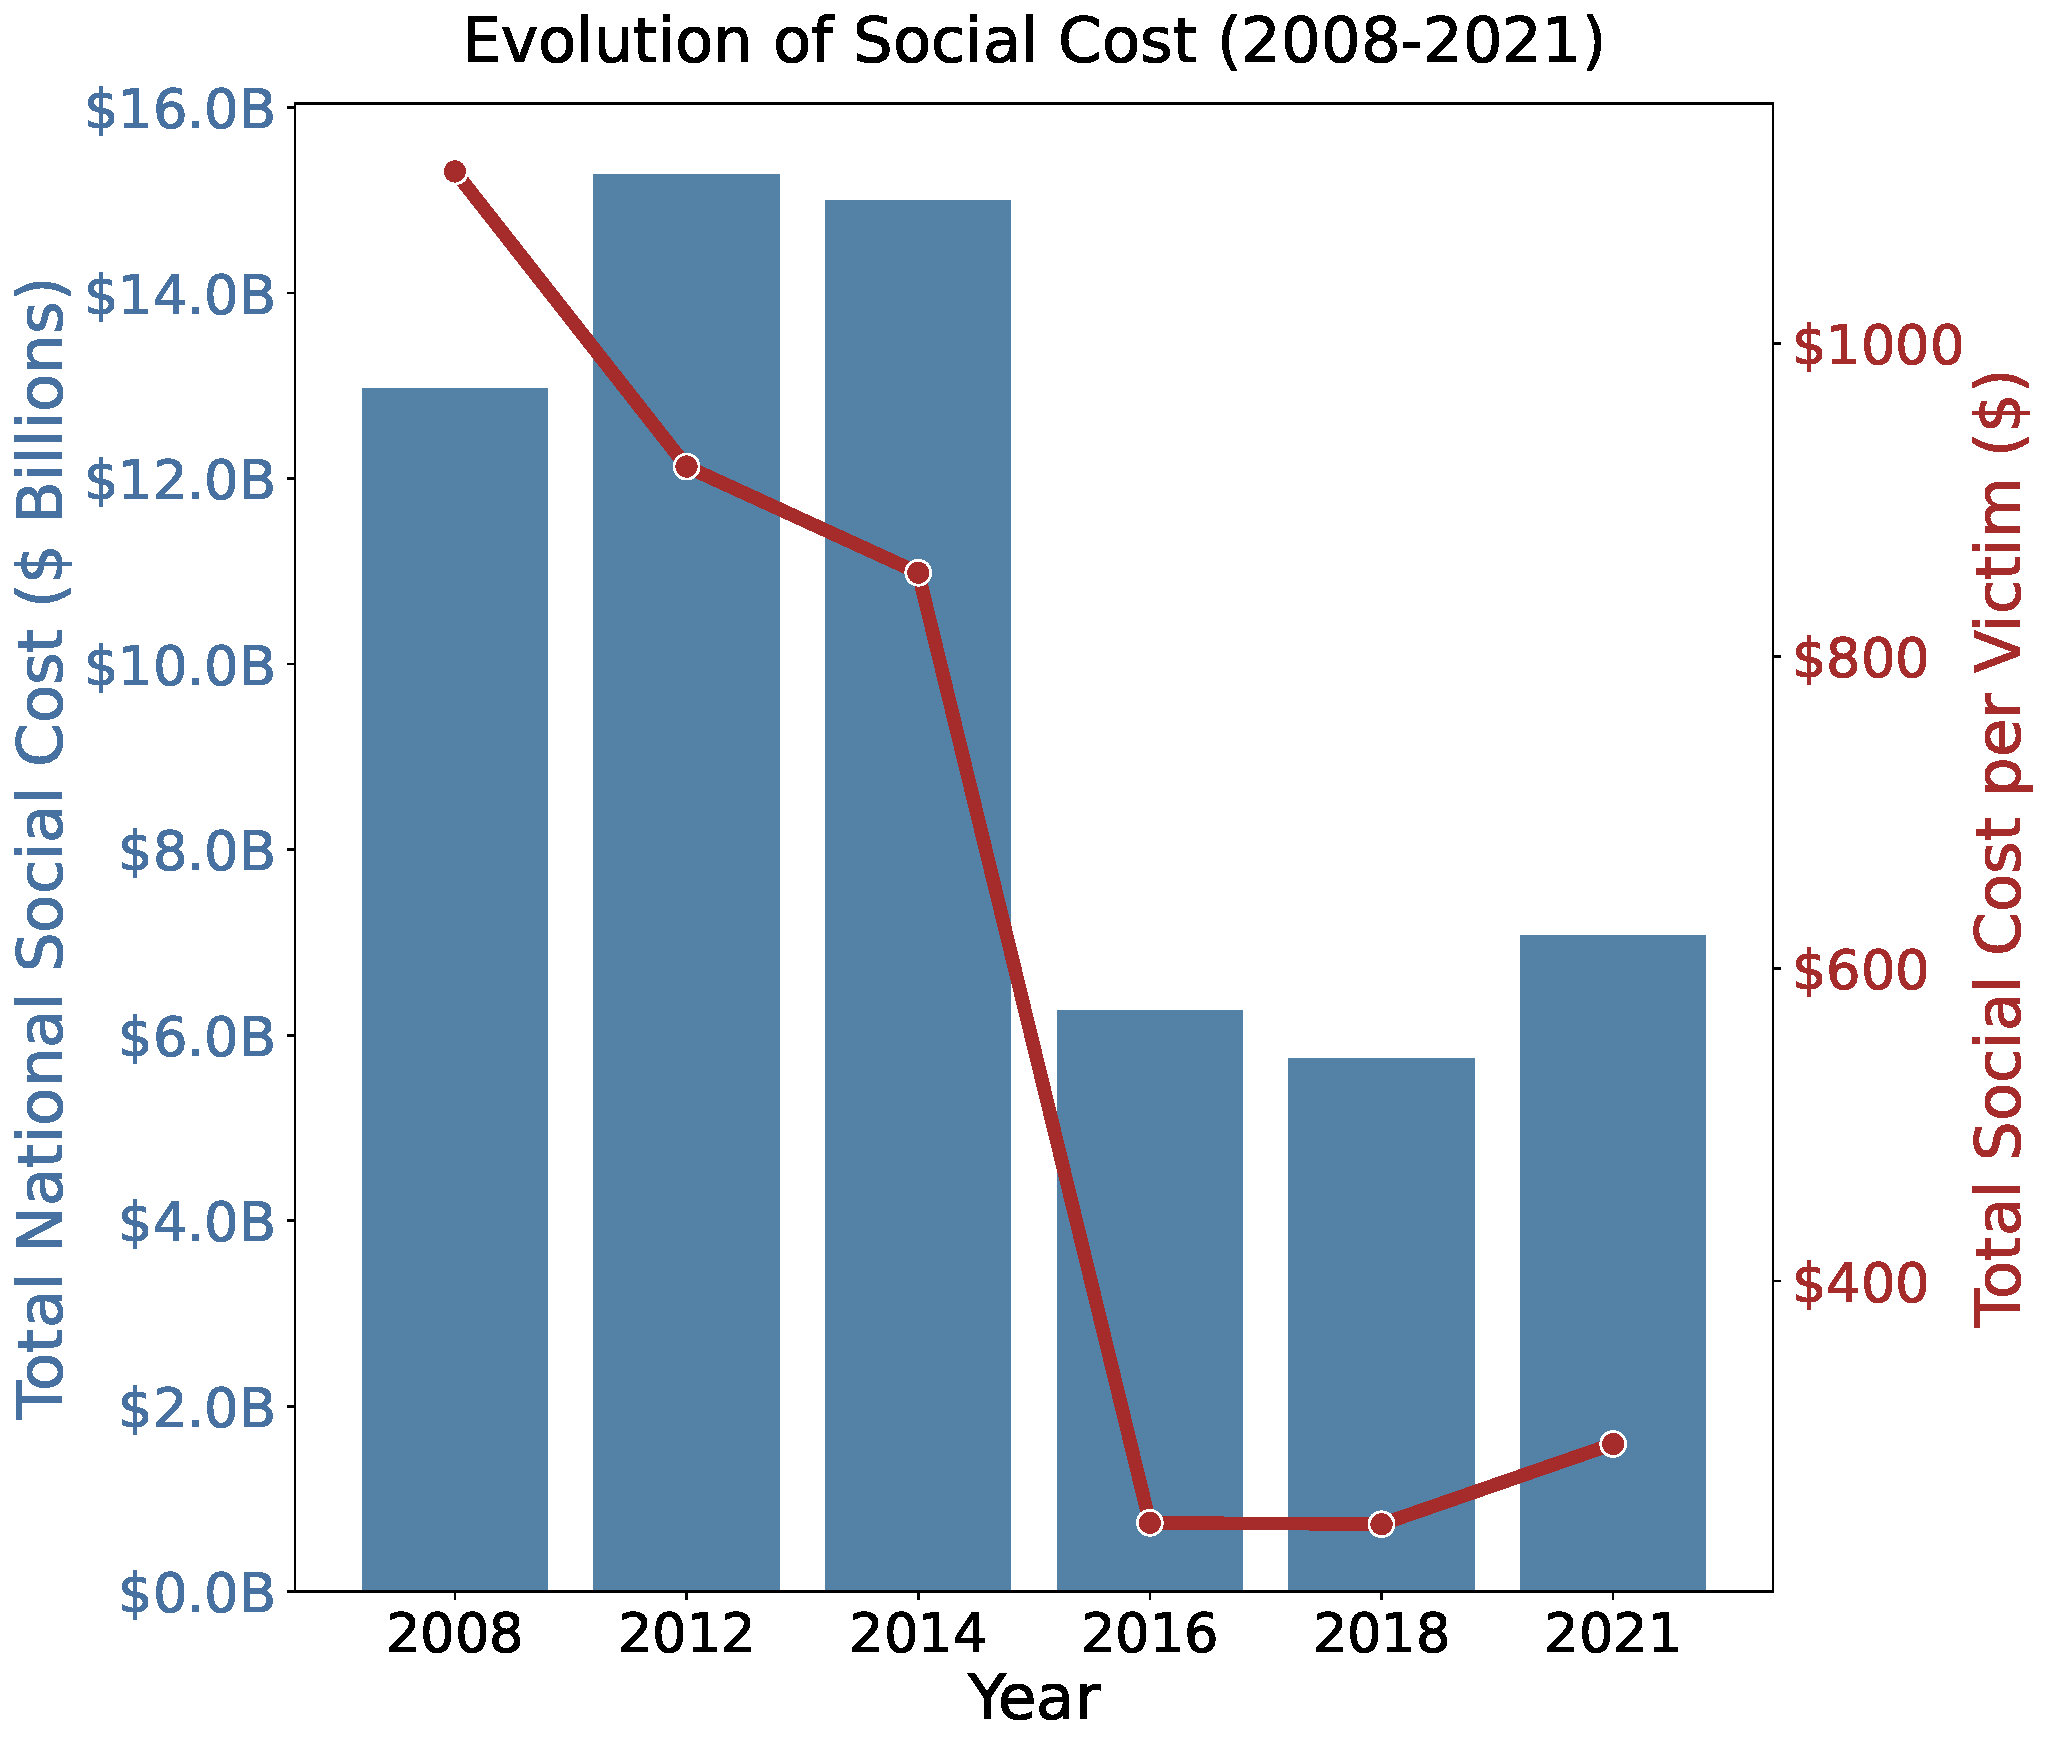
\includegraphics[width=0.45\textwidth]{figures/incident_trends/plot4_social_cost_evolution.pdf}
%     \vspace{-10pt}
%     \caption{Evolution of social costs associated with incidents over the study period.}
%     \label{fig:social_cost_evolution}
%     \vspace{-6pt}
% \end{wrapfigure}

The IDT victim population is presented in Table \ref{tab:victimization_year}, which displays the trend of victimization over time by counting the number of victims in each of the six survey waves. These numbers originate directly from the harmonized ITS dataset previously detailed in Section \ref{sec:data_and_sample}. For each survey wave, the total estimated number of victims (N) was found by summing the final survey weights of all respondents that were confirmed to be successful victims. Each year's weighted \% was then calculated to show its share relative to the total number of victims across all six surveys combined. From Table \ref{tab:victimization_year}, it is clear that the number of victims is generally increasing over time (we refer an interested reader to  Appendices \ref{app:longitudinal} and \ref{app:demographics} for a more detailed trend and demographic analysis).


\begin{table}[ht!]
  \centering
  \begin{minipage}{0.48\textwidth}
    \centering
    \captionof{table}{Victimization by year, from harmonized ITS dataset.}
    \label{tab:victimization_year}
    \begin{tabular}{lrr}
      \toprule
      \textbf{Year} & \textbf{N} & \textbf{\% of dataset} \\
      \midrule
      2008 & 11,684,672 & 9.83 \\
      2012 & 16,580,475 & 13.95 \\
      2014 & 17,576,206 & 14.79 \\
      2016 & 25,563,022 & 21.51 \\
      2018 & 23,536,881 & 19.80 \\
      2021 & 23,928,598 & 20.13 \\
      \bottomrule
    \end{tabular}
  \end{minipage}
    \hfill % Adds spacing between the two minipages
  \begin{minipage}{0.48\textwidth}
    \centering
    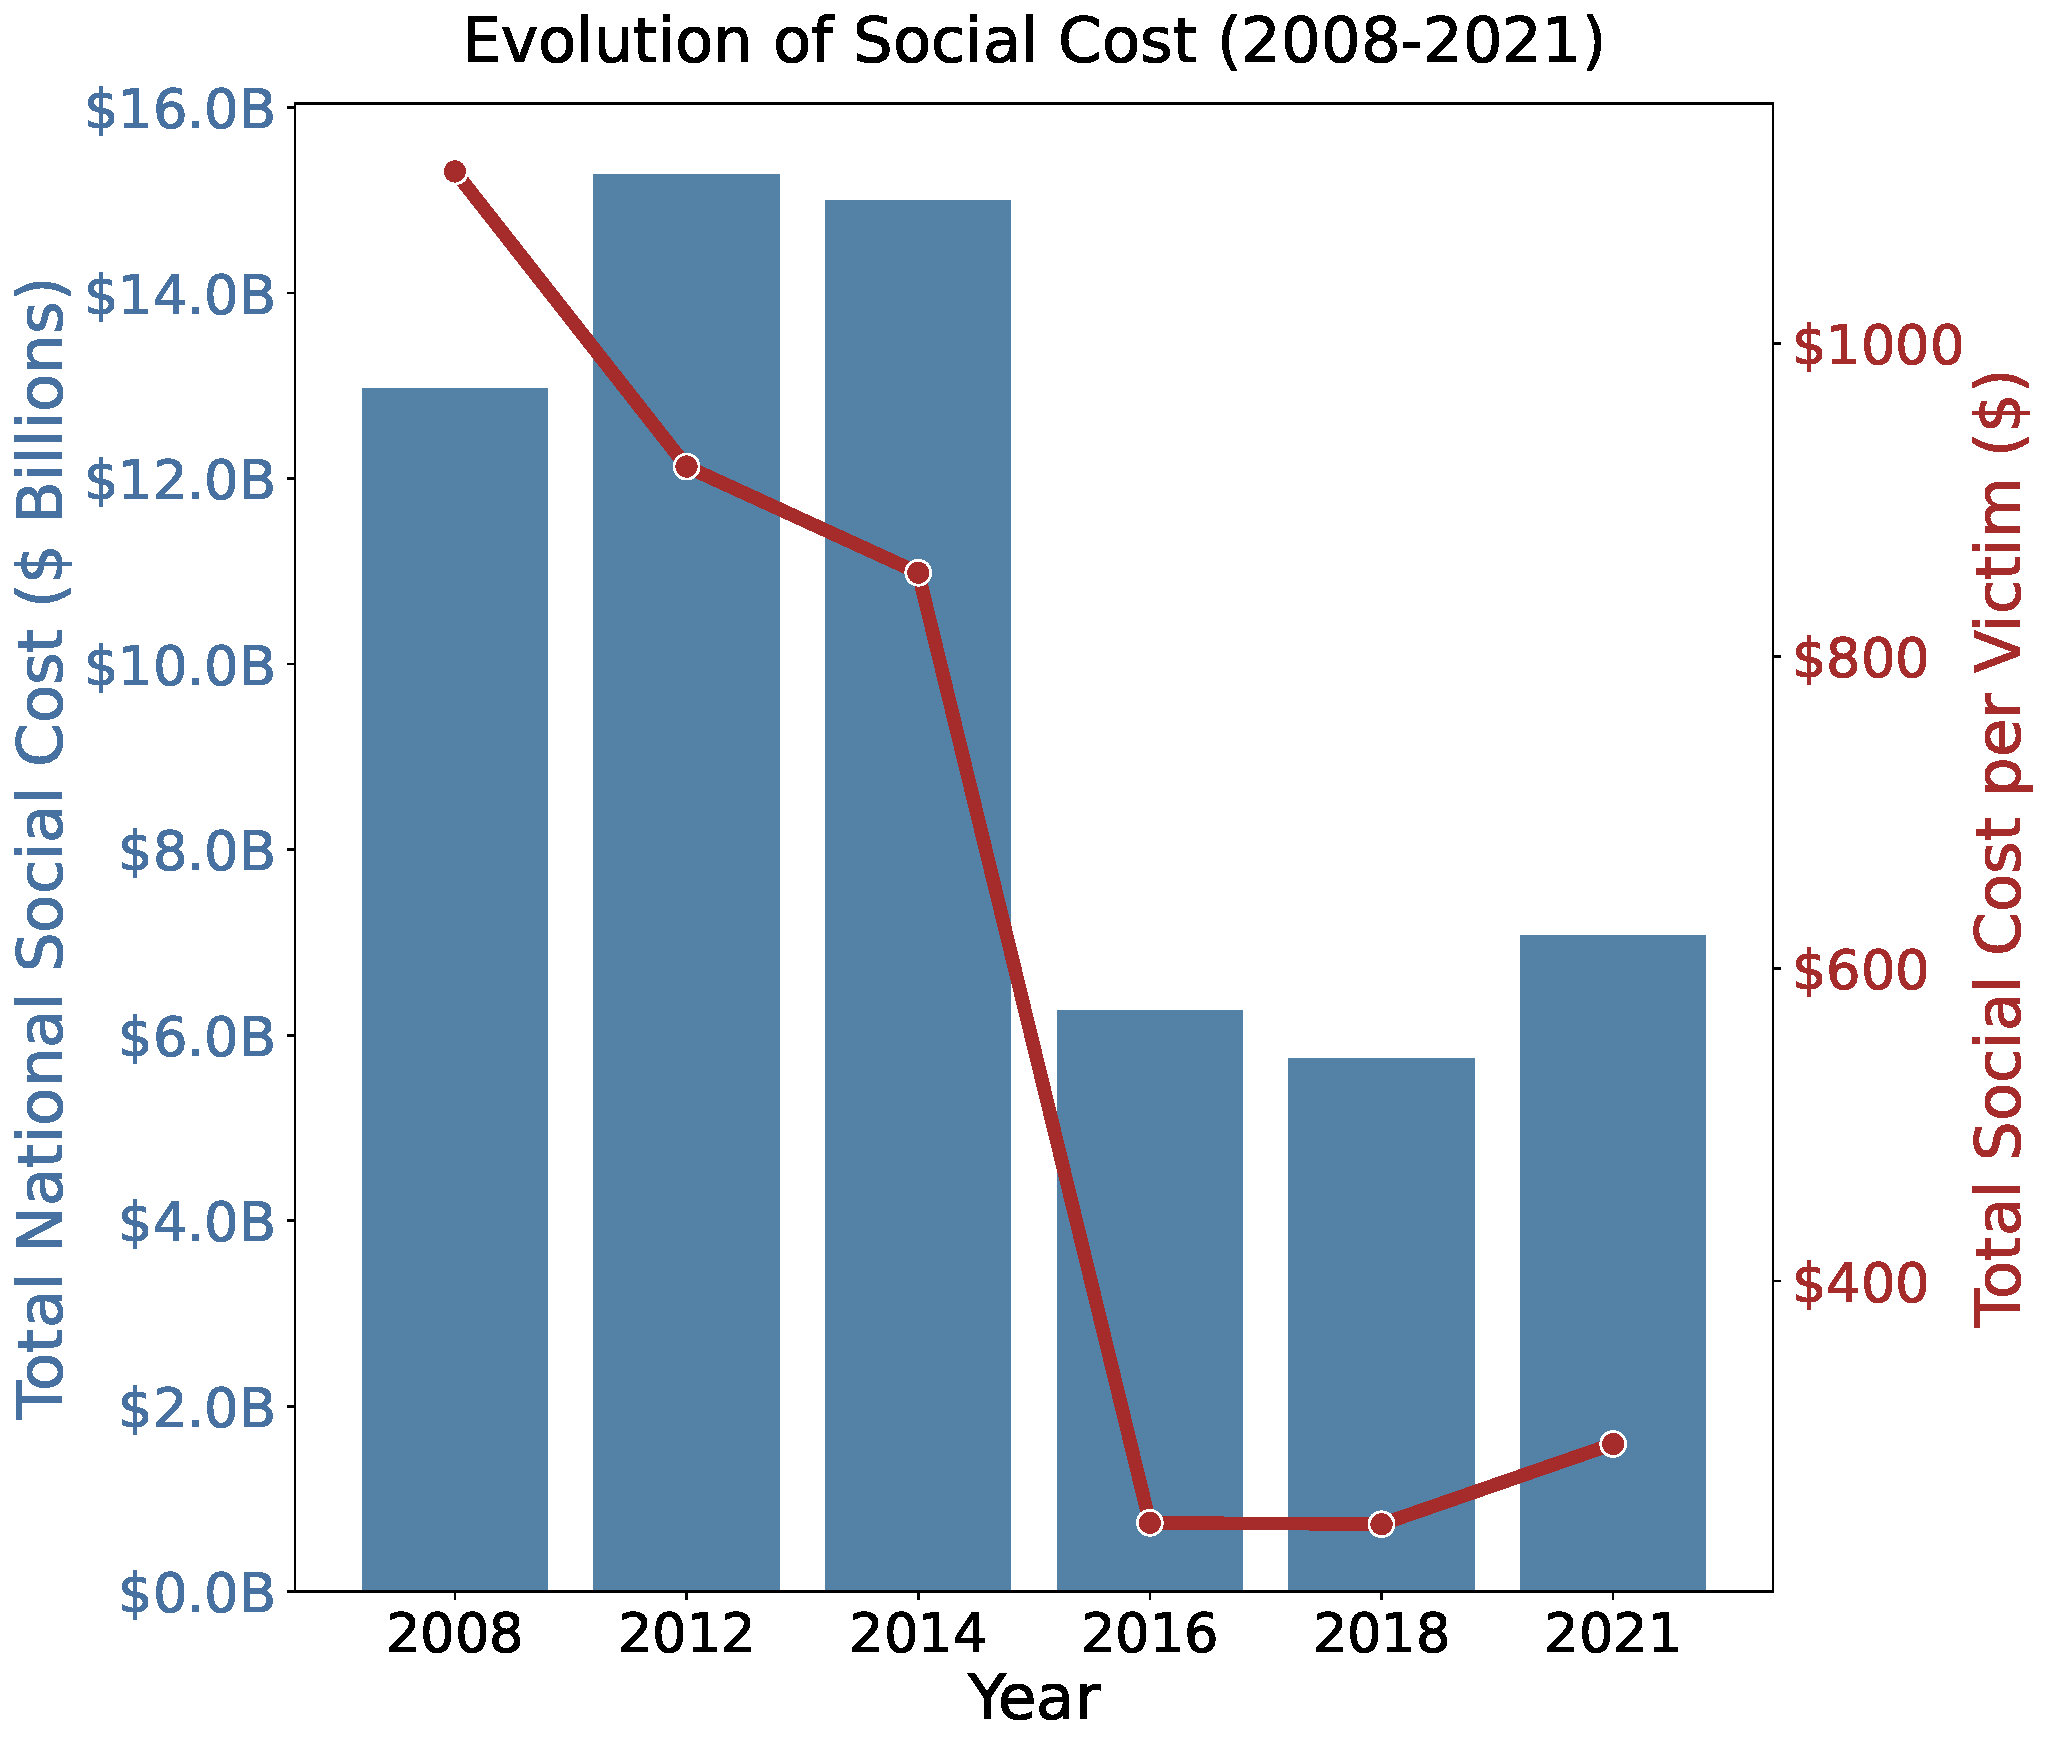
\includegraphics[width=\linewidth]{figures/incident_trends/plot4_social_cost_evolution.pdf}
    \captionof{figure}{Evolution of social costs associated with incidents over the study period.}
    \label{fig:social_cost_evolution}
  \end{minipage}

\end{table}




% \par\vspace{1em} 
% \hrule height 0pt 
% \noindent

% \subsection{Social Cost Model Results}



Next we present the results calculated using our Social Cost model, which monetizes direct financial losses, the opportunity cost of lost time, and healthcare expenses related to physical and emotional distress. Table \ref{tab:social_costs_by_year} displays these calculations. Note that as stated earlier, all monetary values in this table, including average OOP loss, have been adjusted to 2021's inflation. Table \ref{tab:social_costs_by_year} and Figure \ref{fig:social_cost_evolution} reveal two phases of social cost per victim. Between 2008 and 2014, the Total Social Cost per Victim remained high, peaking at \$1,110.31 in 2008. This period was characterized by substantial unrecoverable OOP losses. We observe a dramatic decline in the per-victim cost starting in 2016. The Total Social Cost per Victim fell to approximately \$245 in 2016 and 2018, primarily driven by a sharp reduction in OOP loss (discussed in detail in \ref{sec:trends_in}), and better resolution systems put into place. Despite this per-victim decline, the Total National Social Cost remains a multi-billion dollar problem, totaling over \$7 billion in 2021. This sustained national cost is due to the sheer volume of victims, which reached 23.9 million in the most recent survey wave. 





%\com{Can the sharp drop, or rather discontinuity from 2014 to 2016 again be attributed to the survey methodology change? If so then it is interesting that the trend is arguably going up both before and after the discontinuity..}
%\resp{True, i think the sharp drop is mainly due to the drop in OOP loss, which is probably from the survey methodology change + some effect from EMV. What do you mean the trend is going up before and after? I was thinking the trend is going down before 2016.}


\begin{table}[ht]
\centering
\caption{Social Costs of IDT by Year}
\label{tab:social_costs_by_year}
% Using a smaller font size to help the table fit
\small 
\begin{tabular}{lrrrrrrr}
\toprule
\thead{Year} & 
\thead{Total \\ Weighted \\ Victims} & 
\thead{Avg. Out-of- \\ Pocket Loss (\$)} & 
\thead{Avg. Legal \\ Cost (\$)} & 
\thead{Avg. Lost \\ Time Cost (\$)} & 
\thead{Avg. \\ Healthcare \\ Cost (\$)} & 
\thead{Total Social \\ Cost per \\ Victim (\$)} & 
\thead{Total \\ National \\ Social Cost (\$)} \\
\midrule
\textbf{2008} & 11,684,672 & 747.89 & 5.65 & 355.64 & 1.13 & 1110.31 & 12,973,628,242 \\
\textbf{2012} & 16,580,475 & 679.81 & 3.70 & 236.92 & 0.95 & 921.38 & 15,276,880,586 \\
\textbf{2014} & 17,576,206 & 663.01 & 3.31 & 186.41 & 0.68 & 853.41 & 14,999,689,893 \\
\textbf{2016} & 25,563,022 & 116.43 & 3.21 & 124.97 & 0.66 & 245.27 & 6,269,966,976 \\
\textbf{2018} & 23,536,881 & 117.96 & 1.43 & 124.36 & 0.64 & 244.40 & 5,752,387,938 \\
\textbf{2021} & 23,928,598 & 155.52 & 1.83 & 137.58 & 0.80 & 295.73 & 7,076,429,708 \\
\bottomrule
\end{tabular}
\end{table}


\subsubsection{Trends in Social Cost and Identity Theft}
\label{sec:trends_in}

To better understand the factors affecting the social cost measure, we examine several trends observed from the harmonized ITS data. Below we provide a brief summary of the most important trends, with a more detailed analysis presented in Appendix \ref{app:longitudinal}. 
%
% Considering the types of identity theft experienced, Figure \ref{fig:theft_type_long} shows a shift from traditional financial account misuse to other forms, which is particularly evident in the most recent survey year, 2021. As shown, existing bank account or credit card misuse remain the most common types of identity theft experienced. Misuse of existing credit cards, historically the most prevalent type (affecting over 50\% of victims in some years), saw a substantial decline between 2018 and 2021, dropping to roughly 38\%. Existing bank account misuse followed a similar pattern, also decreasing significantly in 2021. In contrast, the category of "Other Existing Account Misuse," which includes misuse of online accounts like email or social media, experienced a dramatic surge in 2021, rising from around 10\% in 2018 to over 30\% of victims in 2021. This indicates a significant change in criminal activity towards compromising online credentials. This could also be due to the rapid rise of social media over the \rev{last few years}. New account fraud and other misuses of personal information remained relatively stable at lower prevalence levels throughout the period.
%
%
% \begin{figure}[htbp]
%     \centering
%     % --- Subfigure A: Counts ---
%     \begin{subfigure}[b]{0.48\textwidth}
%         \centering
%         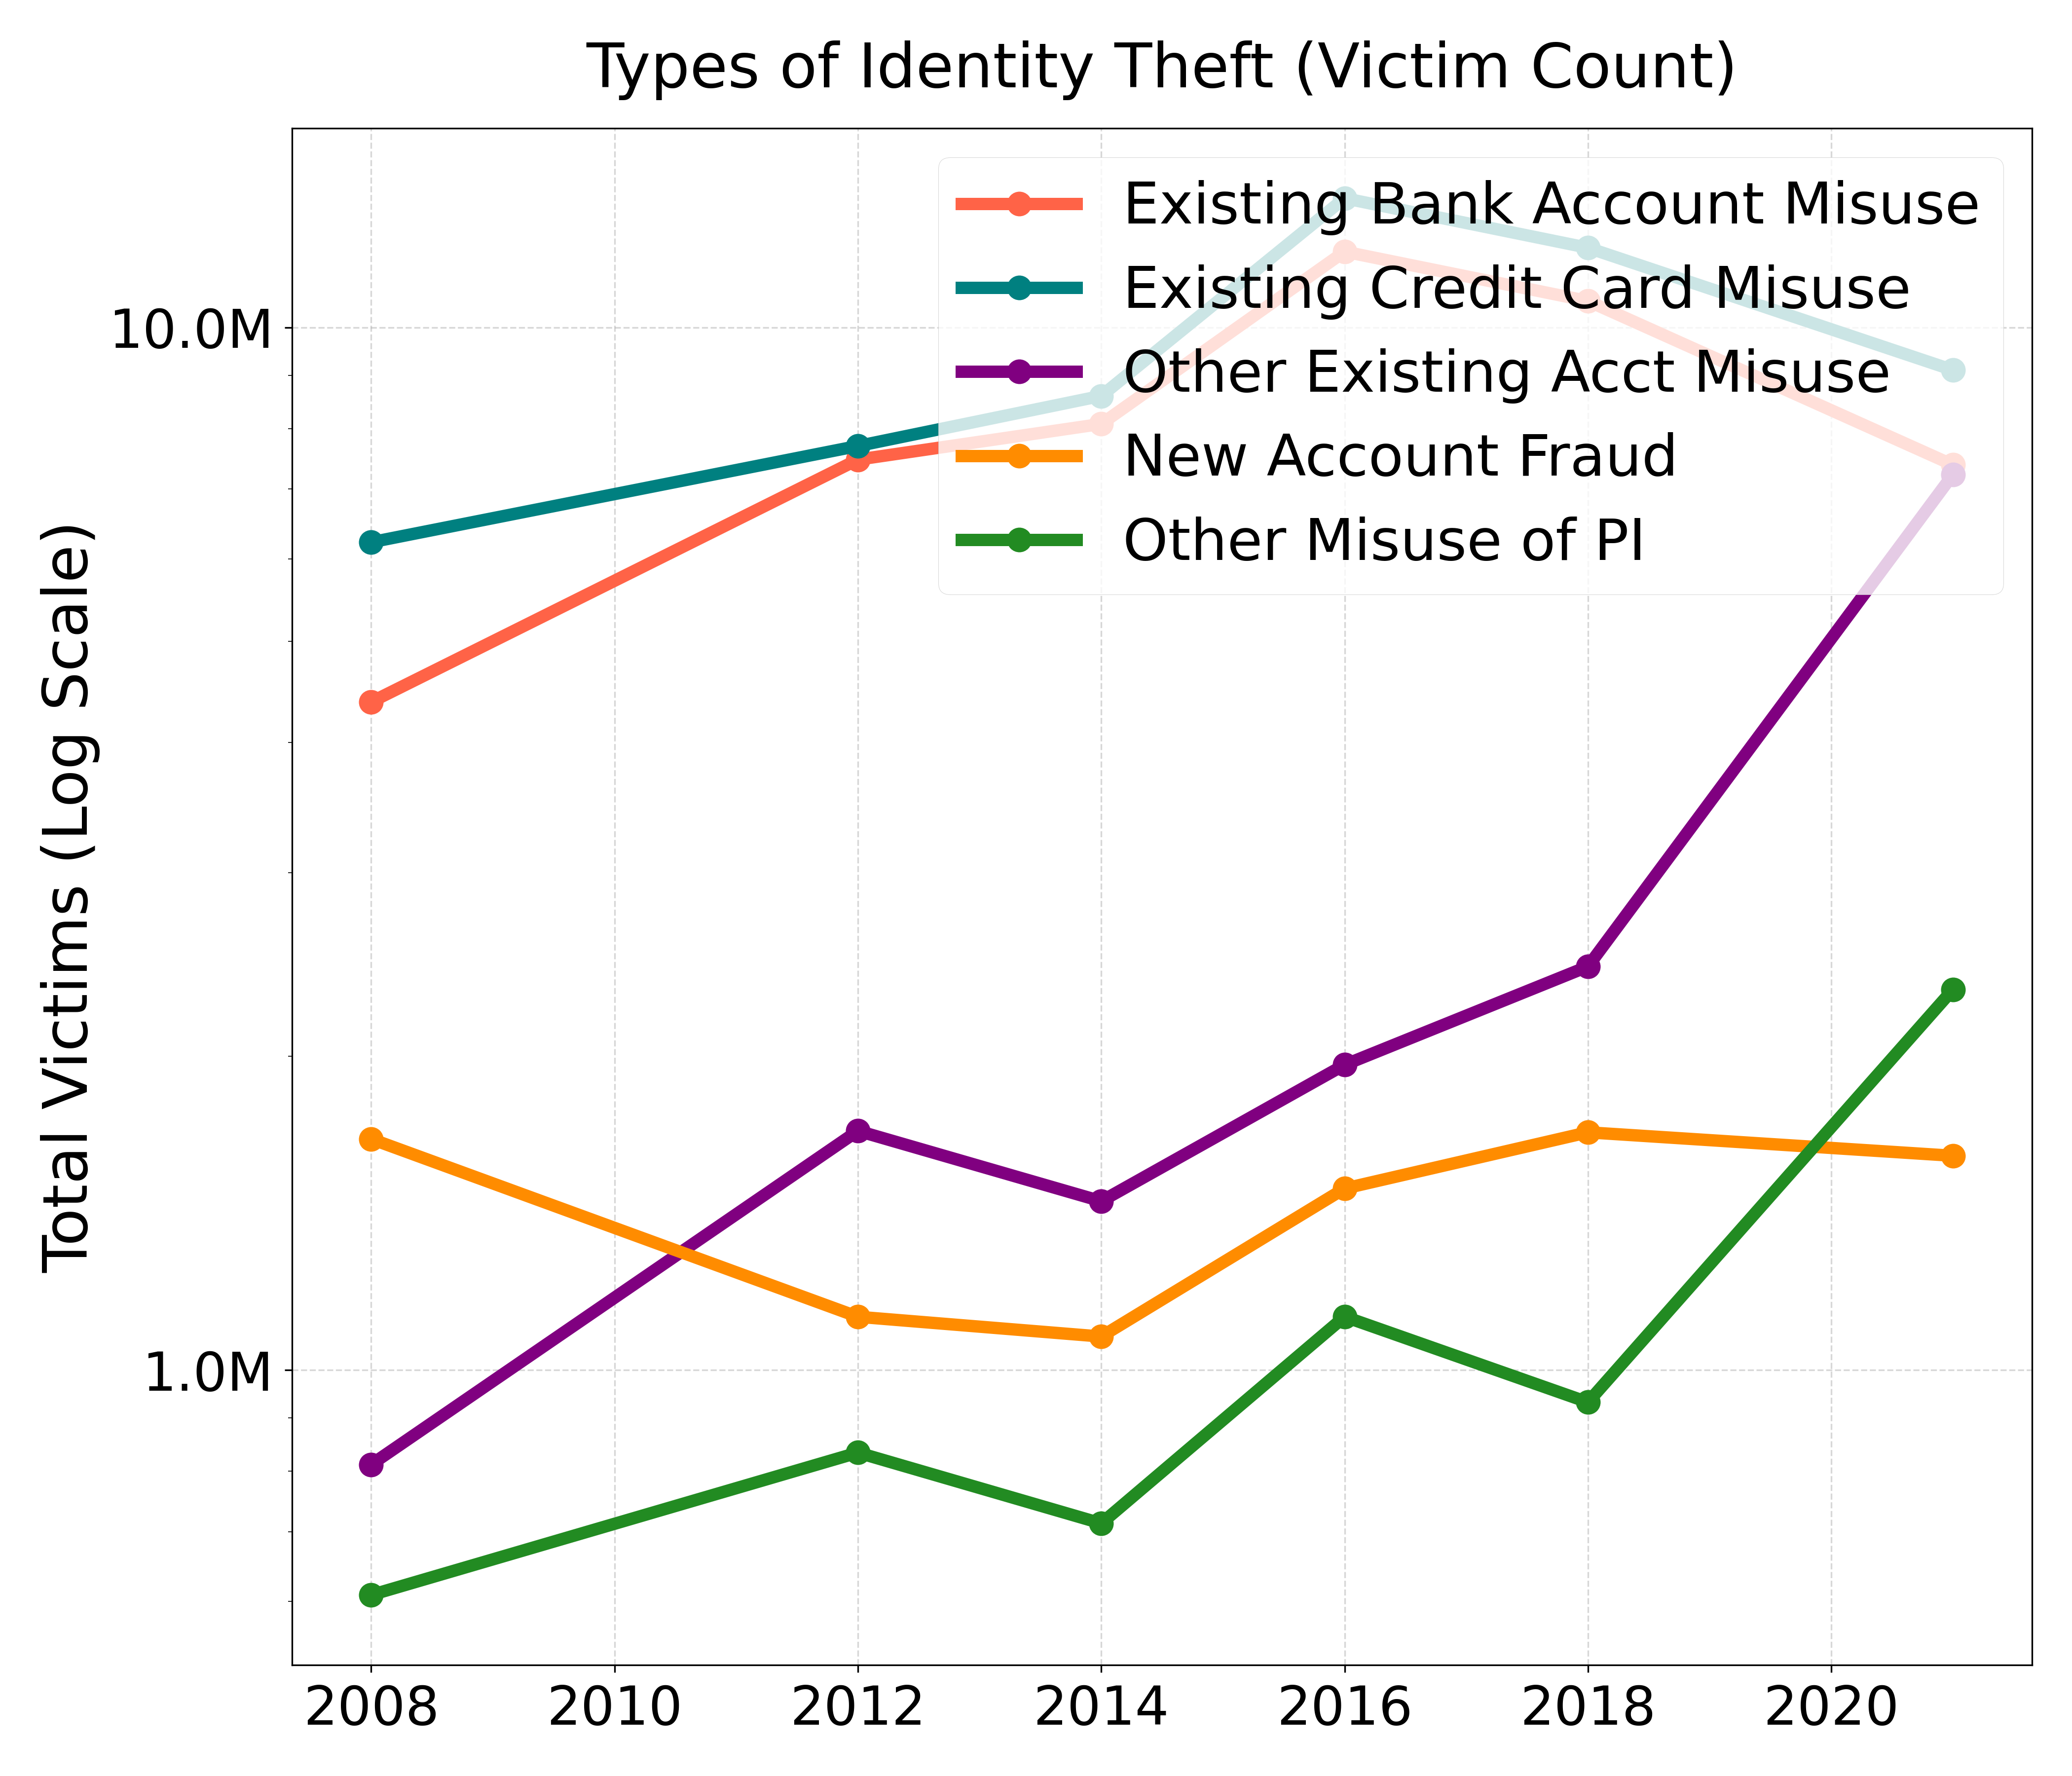
\includegraphics[width=\textwidth]{figures/incident_trends/plot2_theft_types_count.png}
%         \caption{Number of victims categorized by the type of identity theft they suffered from.}
%         \label{fig:theft_type_long_a}
%     \end{subfigure}
%     \hfill
%     % --- Subfigure B: Percentages ---
%     \begin{subfigure}[b]{0.48\textwidth}
%         \centering
%         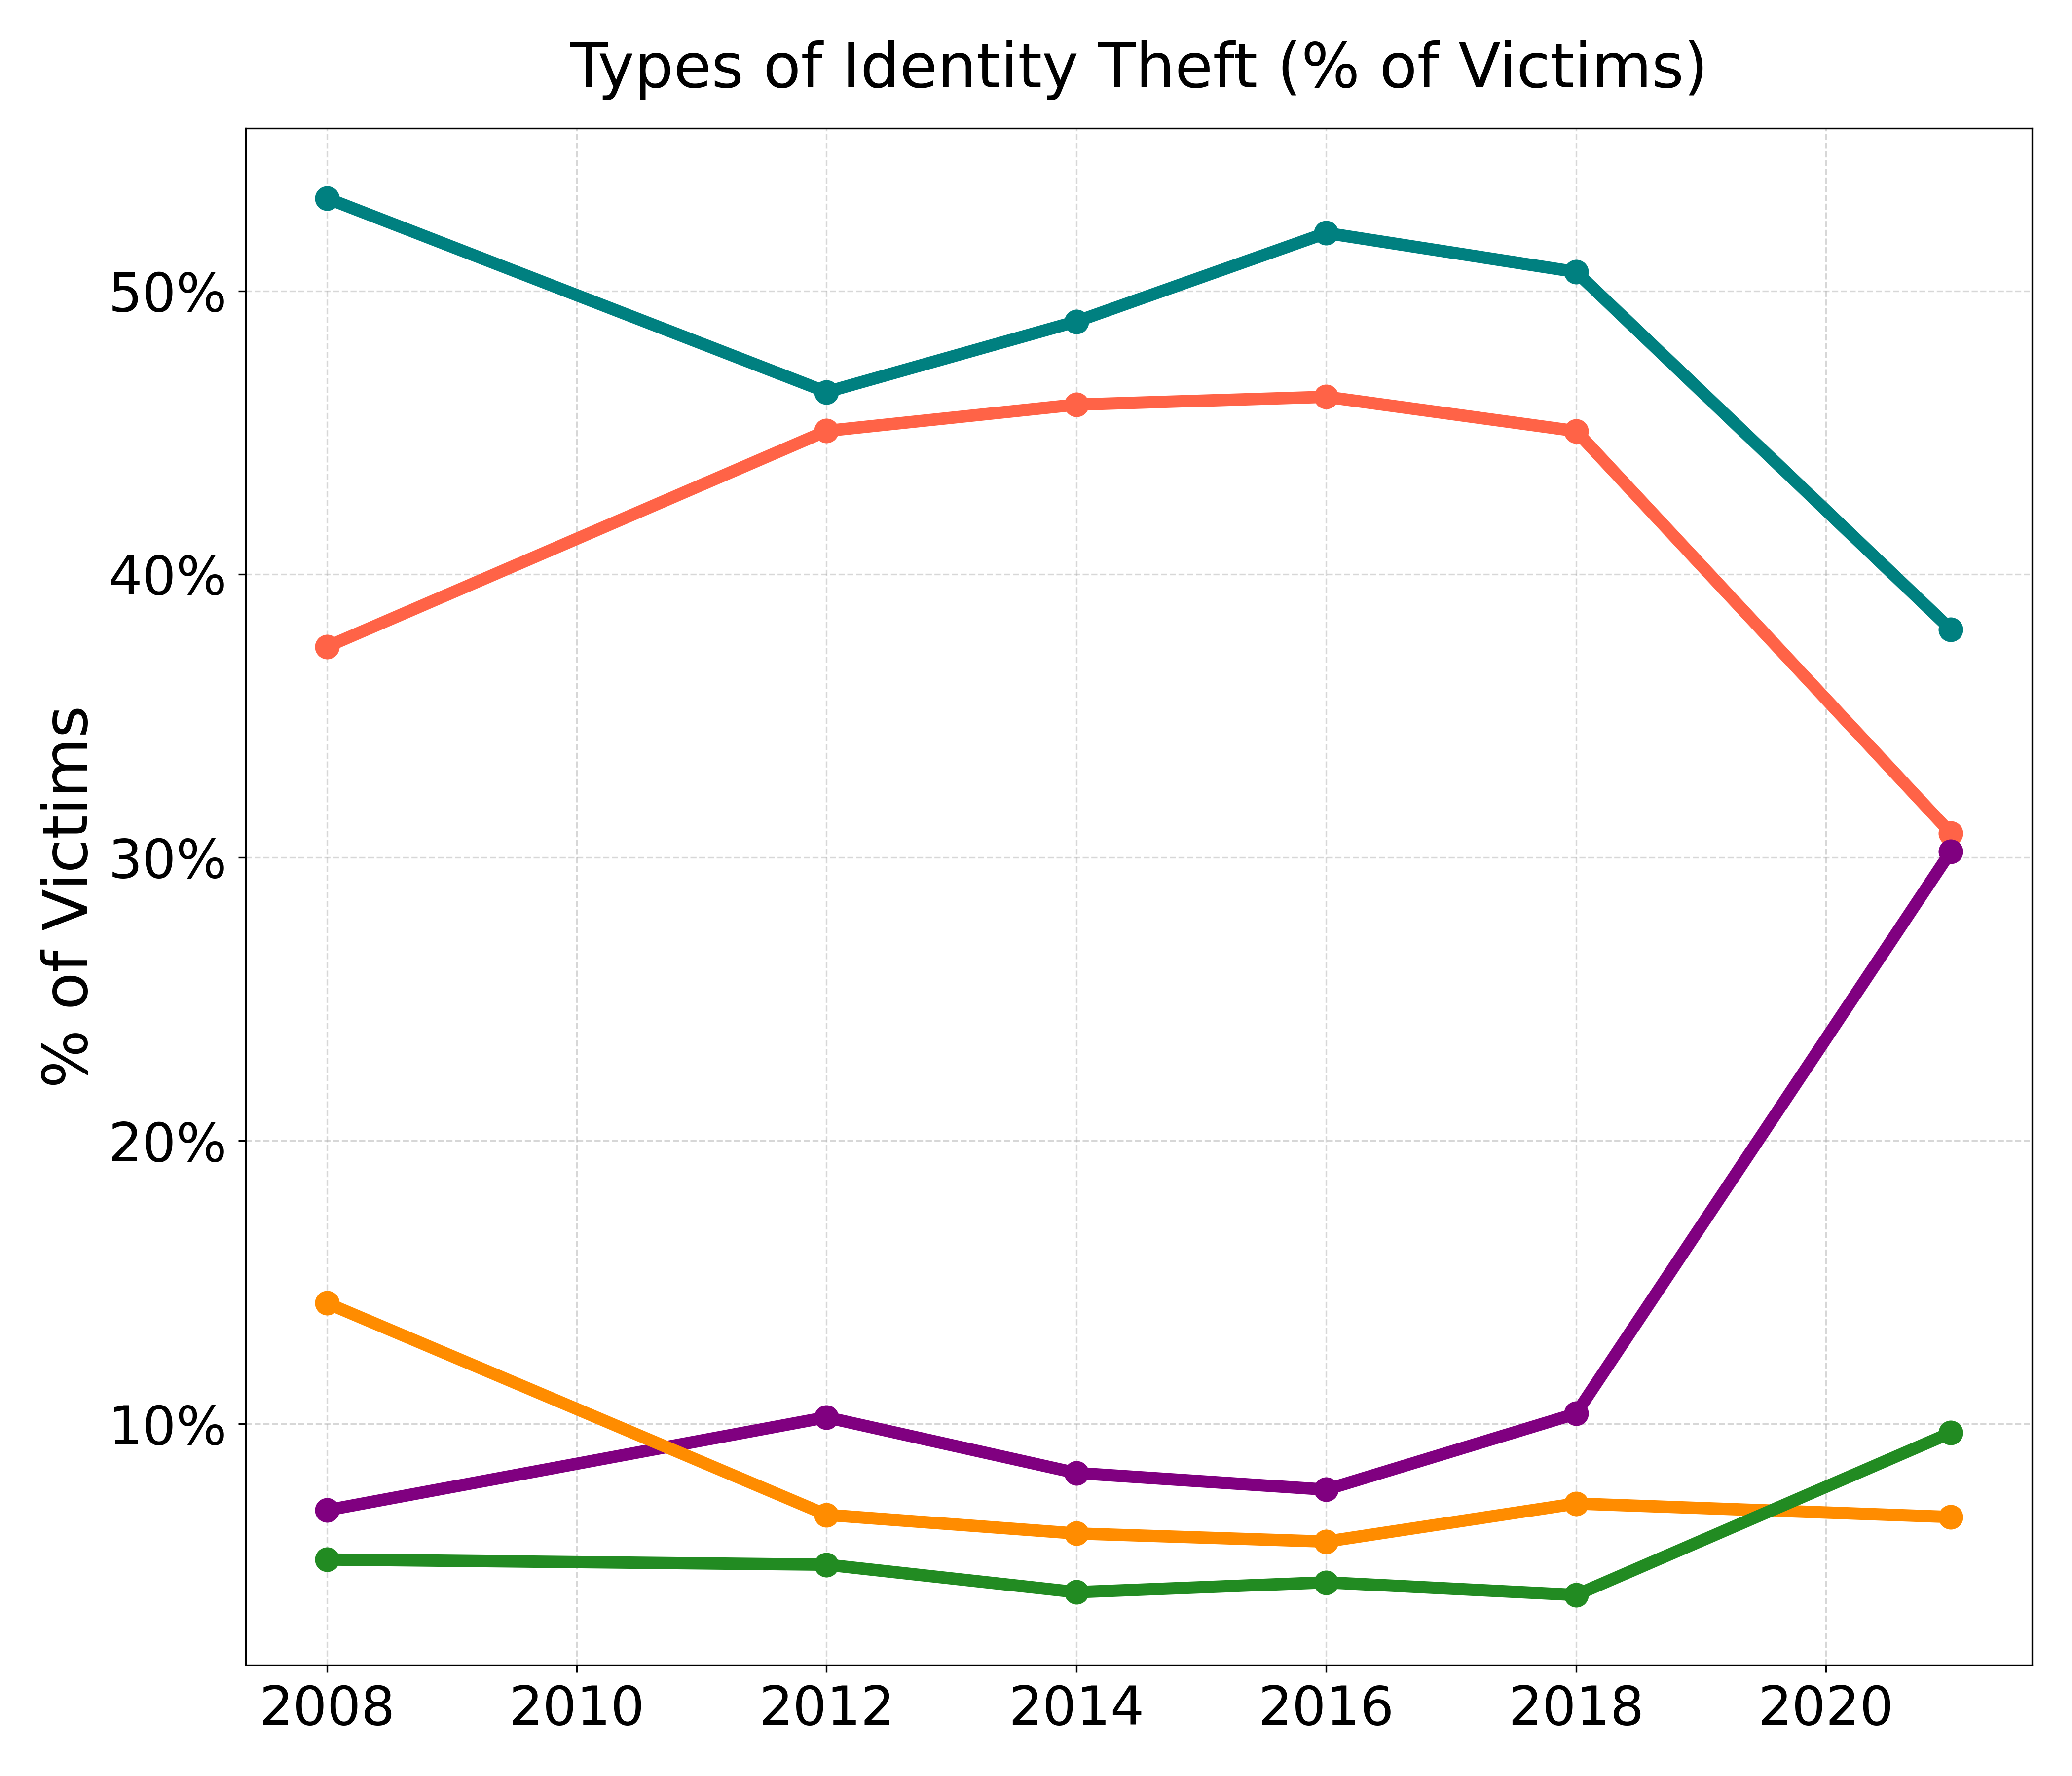
\includegraphics[width=\textwidth]{figures/incident_trends/plot2_theft_types_percentage.png}
%         \caption{Percentage of victims categorized by the type of identity theft they suffered from.}
%         \label{fig:theft_type_long_b}
%     \end{subfigure}
    
%     \caption{Analysis of theft types over the longitudinal study period.}
%     \label{fig:theft_type_long}
% \end{figure}


\begin{figure}[htbp]
    \centering
    % --- Subfigure A: Counts ---
    \begin{subfigure}[b]{0.48\textwidth}
        \centering
        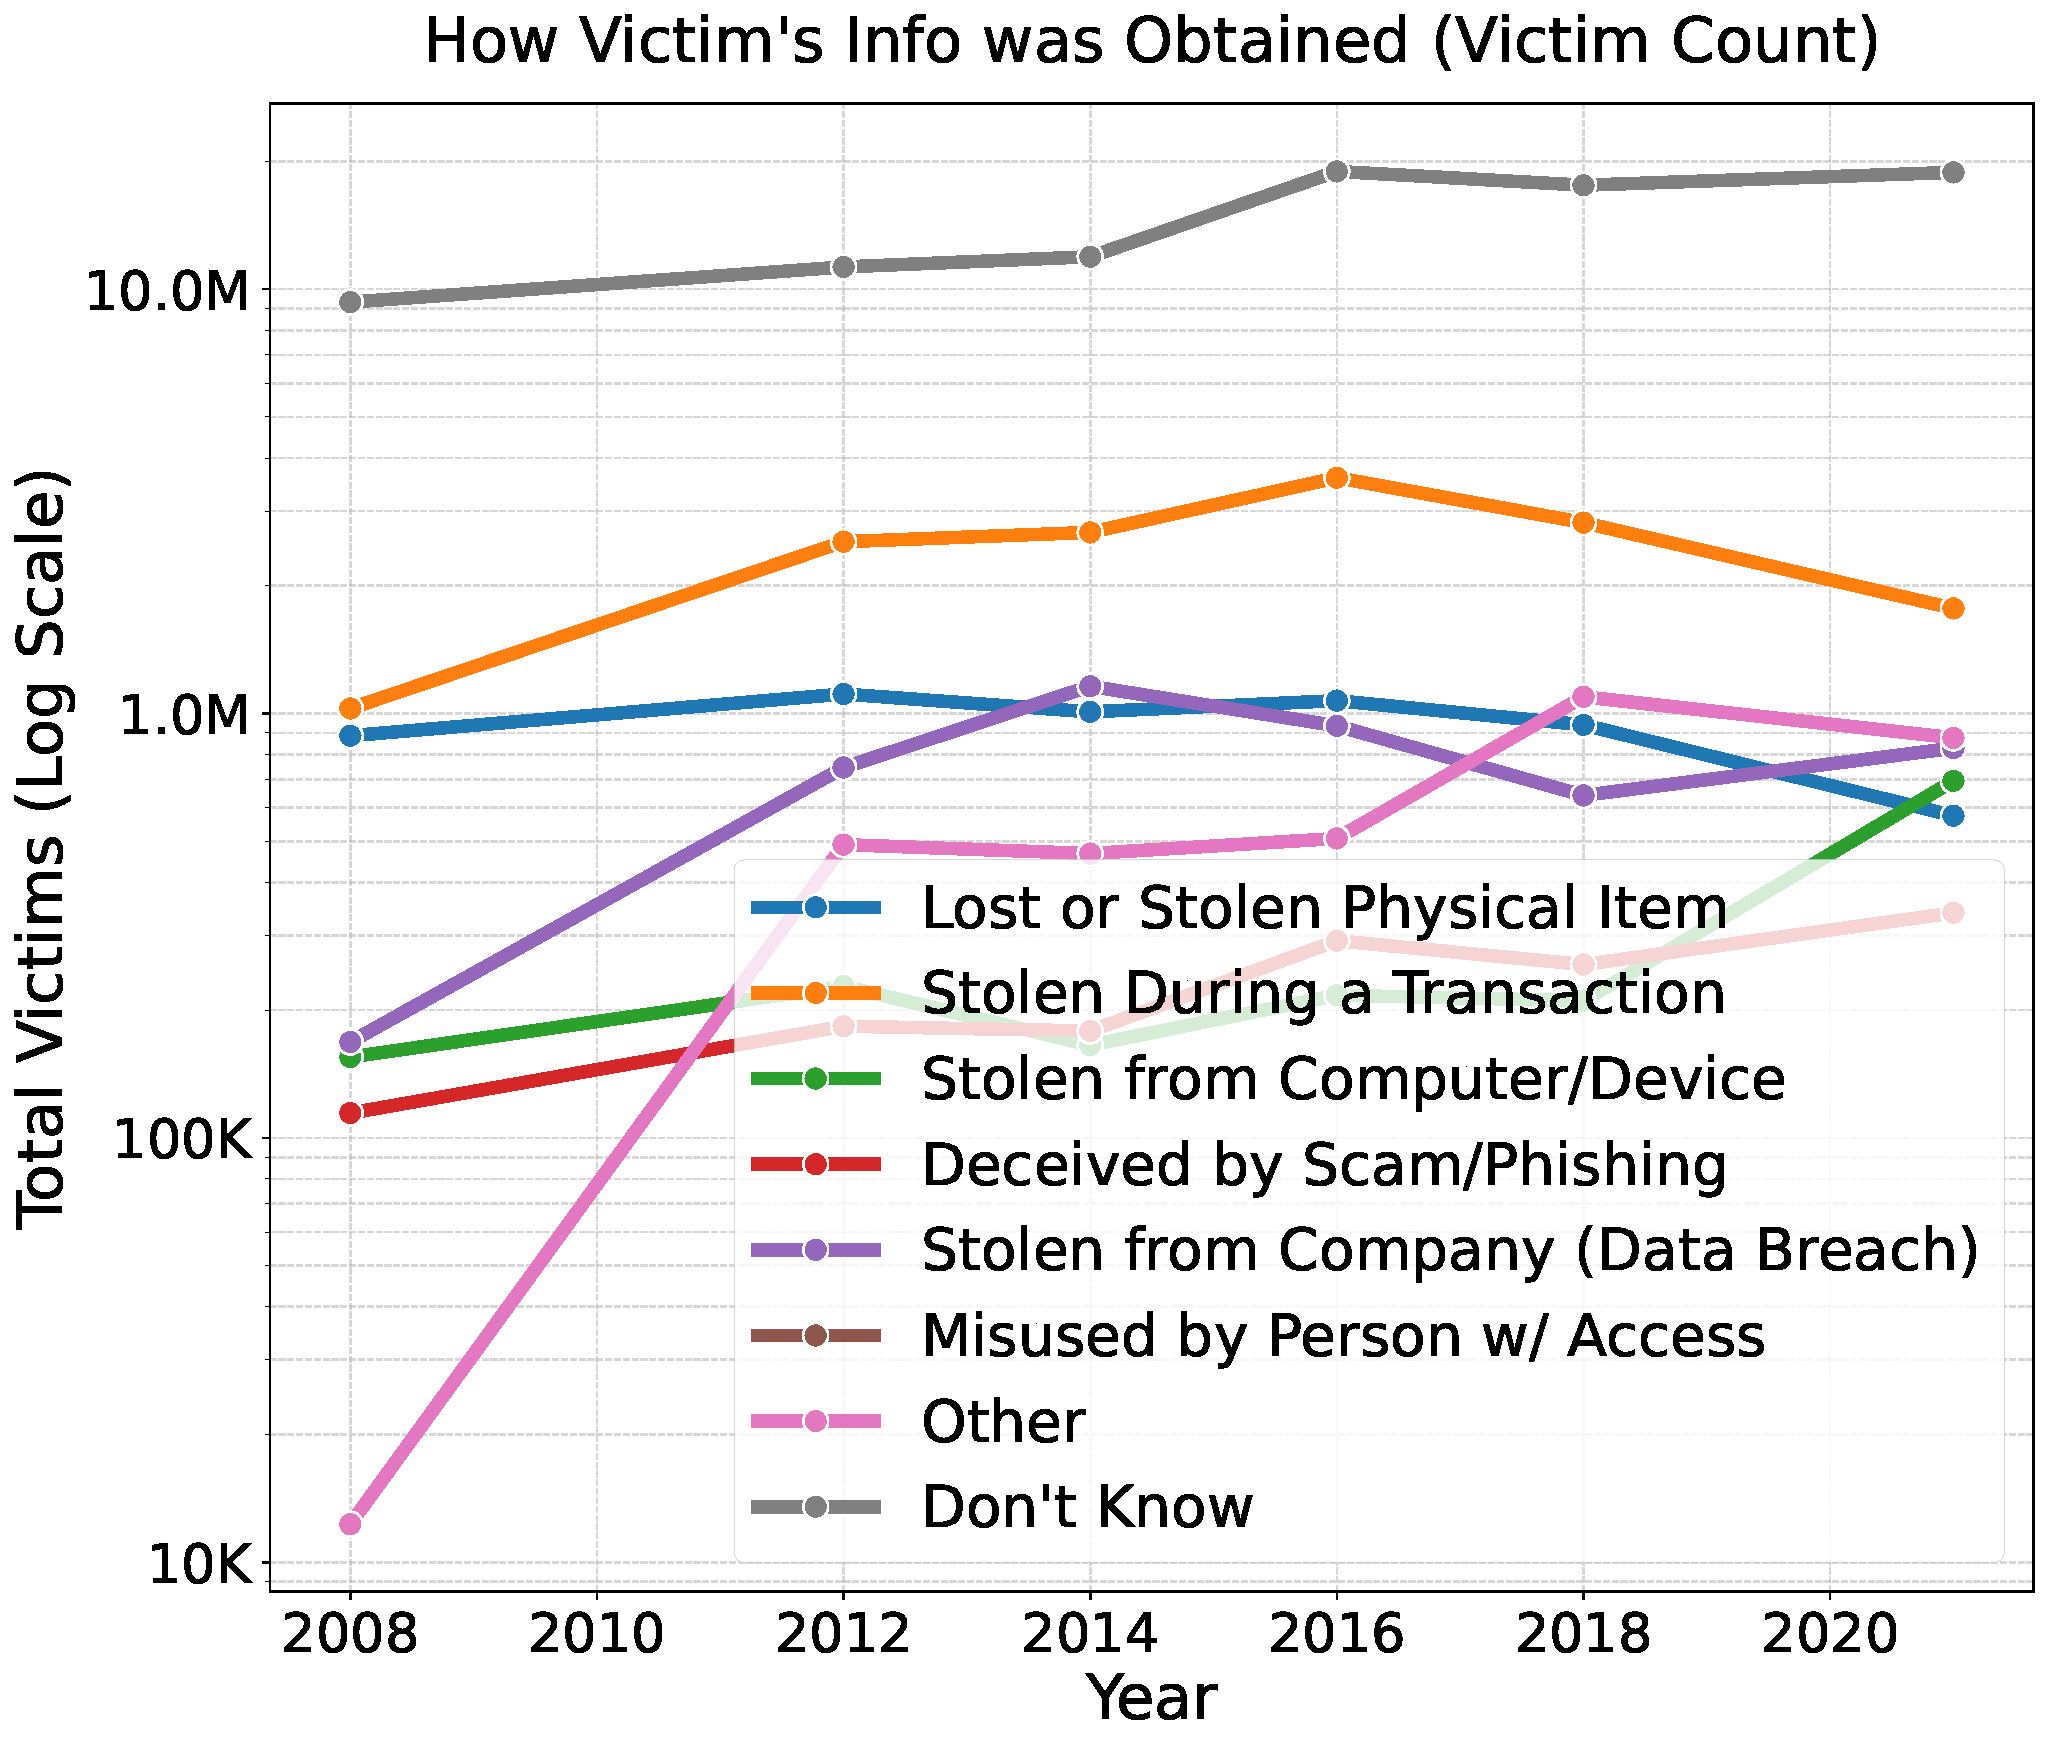
\includegraphics[width=\textwidth]{figures/incident_trends/plot1_theft_methods_count.pdf}
        \caption{Number of victims categorized by how their information was stolen.}
        \label{fig:theft_method_long_a}
    \end{subfigure}
    \hfill % Adds horizontal space between the two images
    % --- Subfigure B: Percentages ---
    \begin{subfigure}[b]{0.48\textwidth}
        \centering
        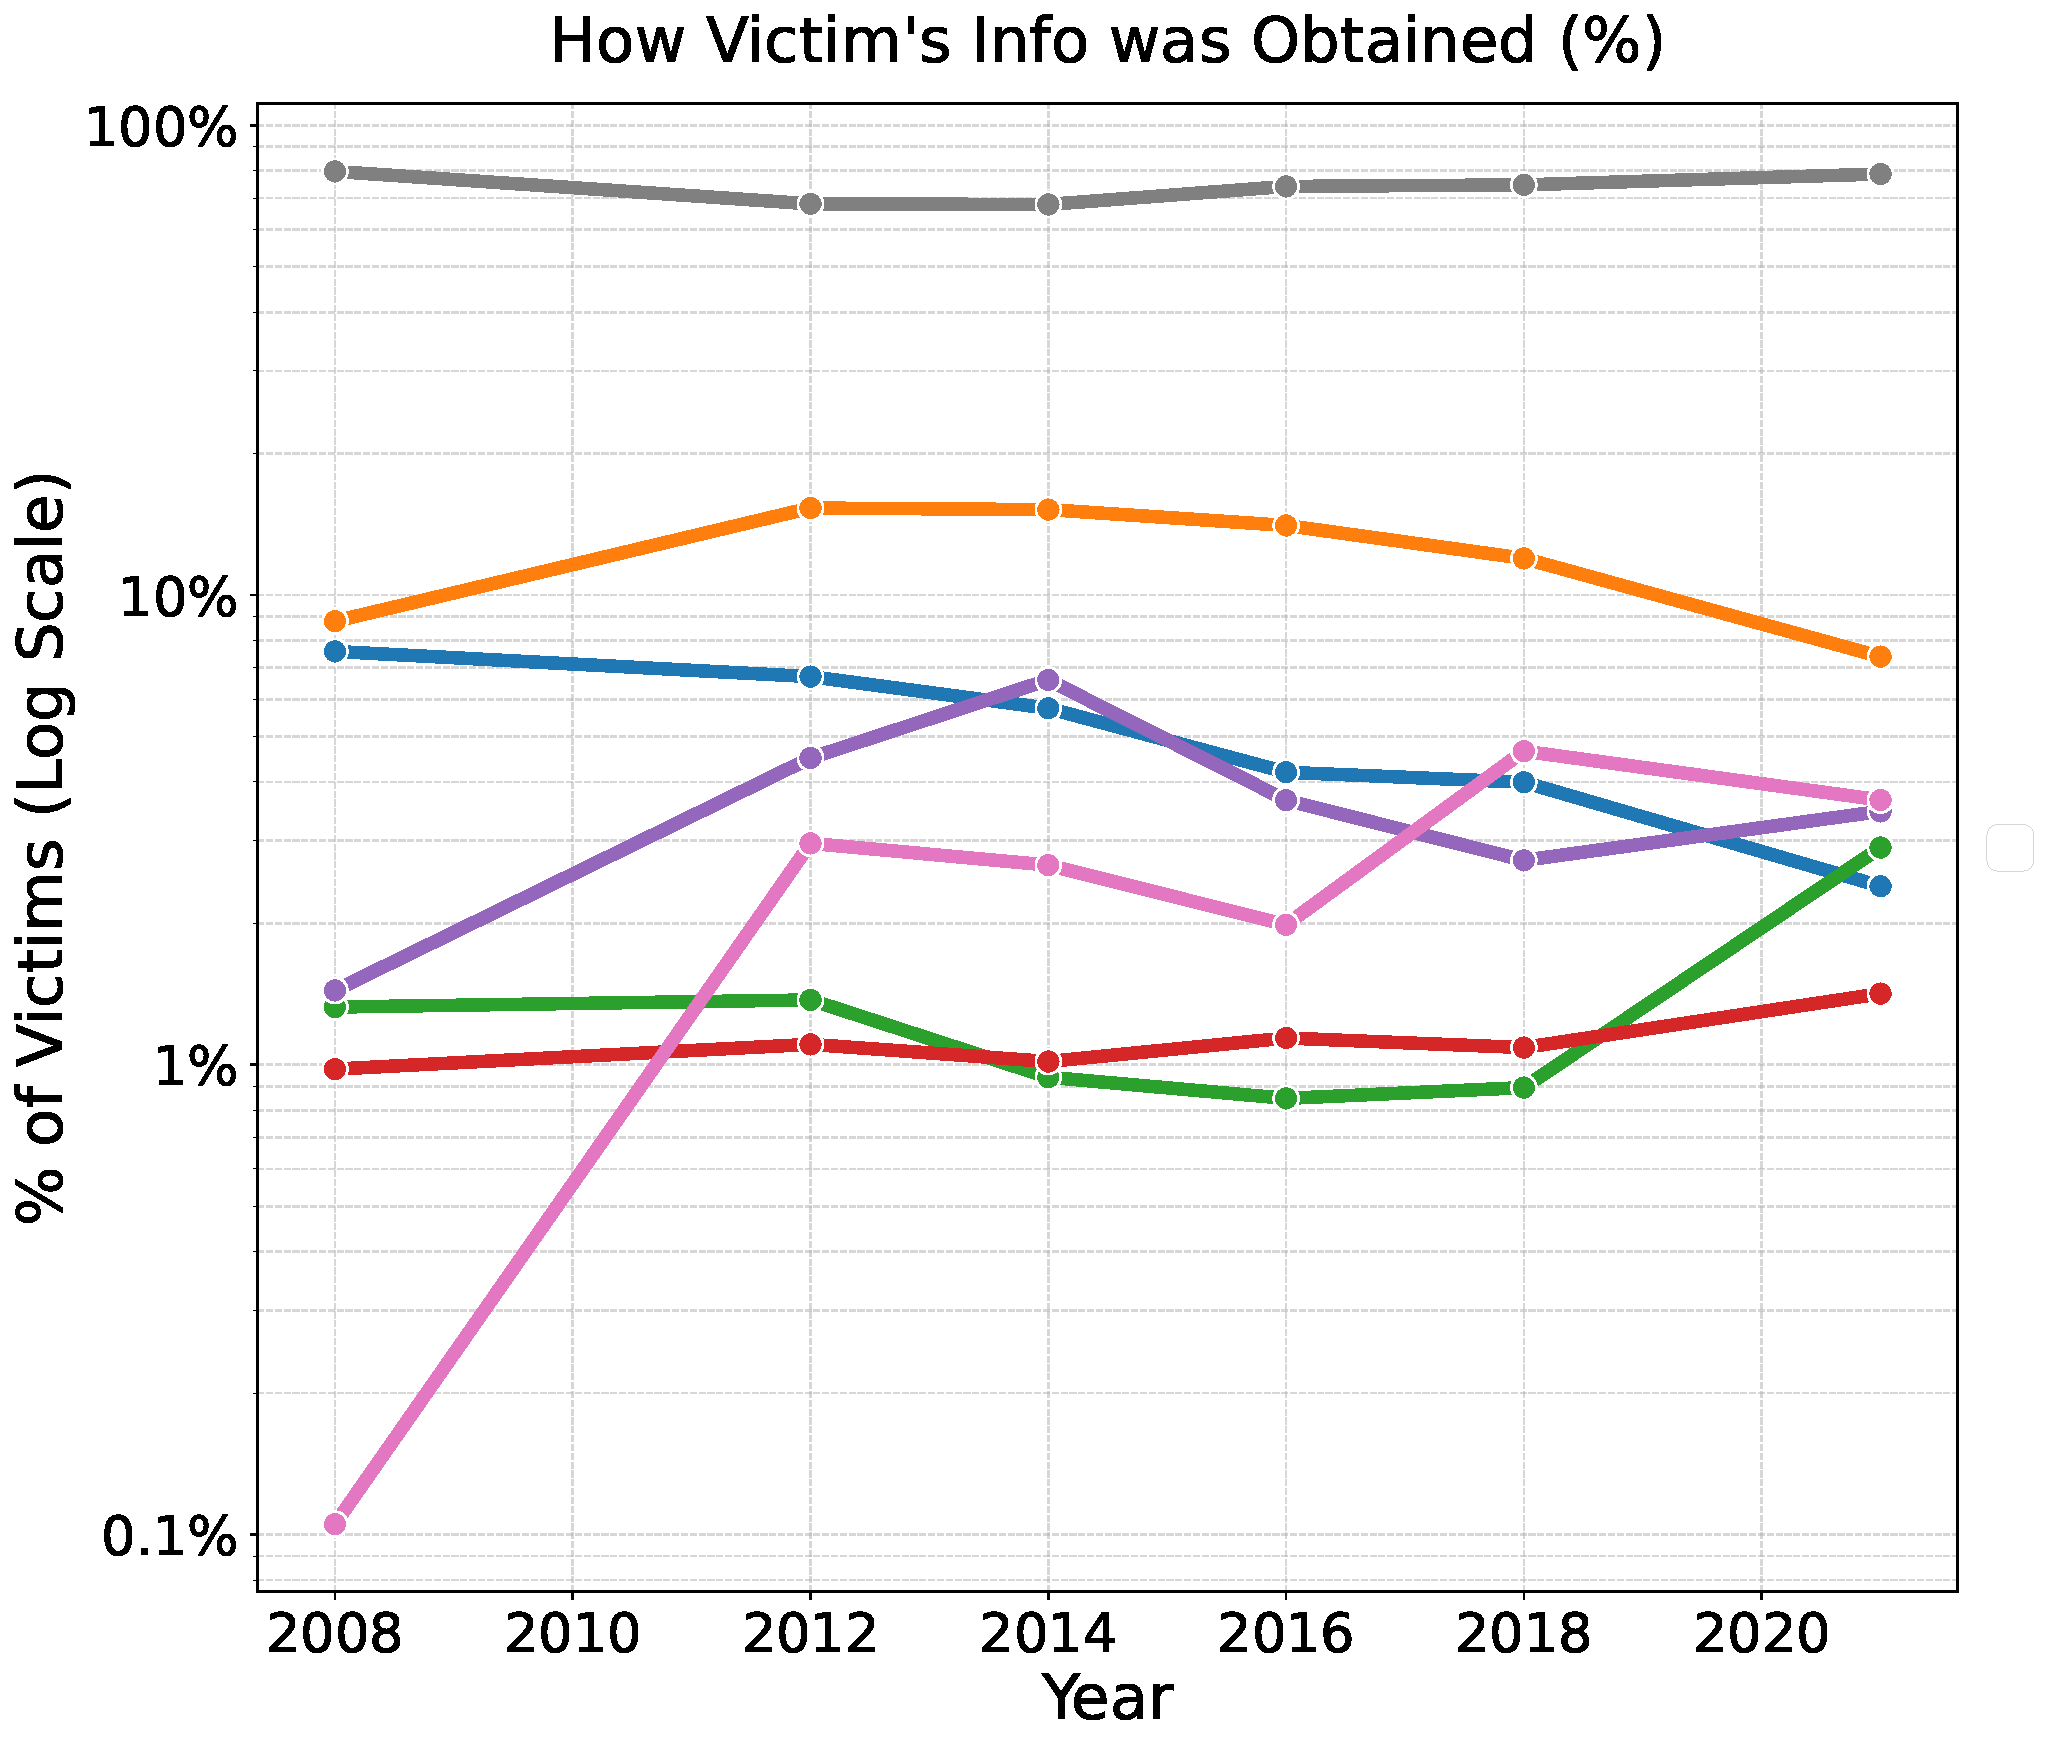
\includegraphics[width=\textwidth]{figures/incident_trends/plot1_theft_methods_percentage.pdf}
        \caption{Percentage of victims categorized by how their information was stolen.}
        \label{fig:theft_method_long_b}
    \end{subfigure}
    
    \caption{Analysis of theft methods over the longitudinal study period.}
    \label{fig:theft_method_long}
\end{figure}

Figure \ref{fig:theft_method_long} displays how victims reported their information was obtained by offenders, which adds more context to the nature of the crime they suffered. A noticeable trend is the considerable decline in information being compromised during a transaction. This method, although still the most common means of identified theft, peaked in 2012 and 2014, and then fell sharply after, accounting for less than 8\% in 2021. Note that in October 2015, the major credit card networks (Europay, MasterCard, and Visa) implemented the EMV liability shift, a policy change that transferred financial responsibility for in-person counterfeit card fraud from the card issuer to whichever party in the transaction (either the merchant or the issuer) had not adopted the more secure chip card technology \cite{CRS_EMV_2016}. This was not a government mandated law but rather a policy change by the major credit card networks to financially incentivize the adoption of chip technology. The policy forced a nationwide payment infrastructure upgrade in an effort to counter the vulnerability of the easily cloned magnetic strip, which had been a leading carrier of counterfeit card fraud. The EMV liability shift was a major turning point in the fight against in-person payment fraud. The reduction in information being stolen during a transaction in Figure \ref{fig:theft_method_long} aligns with the time frame of the October 2015 liability shift for EMV chip card adoption in the United States. The efficacy of this transition was reported by the Federal Reserve, which reported that in-person card fraud, including counterfeit cards, declined from \$3.68 billion in 2015 to \$2.91 billion in 2016 \cite{fed2018fraud}. Similarly, Visa also reported that by October 2016, counterfeit fraud dollars at chip-enabled merchants had dropped by 43\% compared to a year earlier \cite{visa2016infographic}, and later data showed this decline reached 66\% by June 2017 \cite{visa2017report}.

\begin{wrapfigure}{r}{0.5\textwidth}
    \centering
    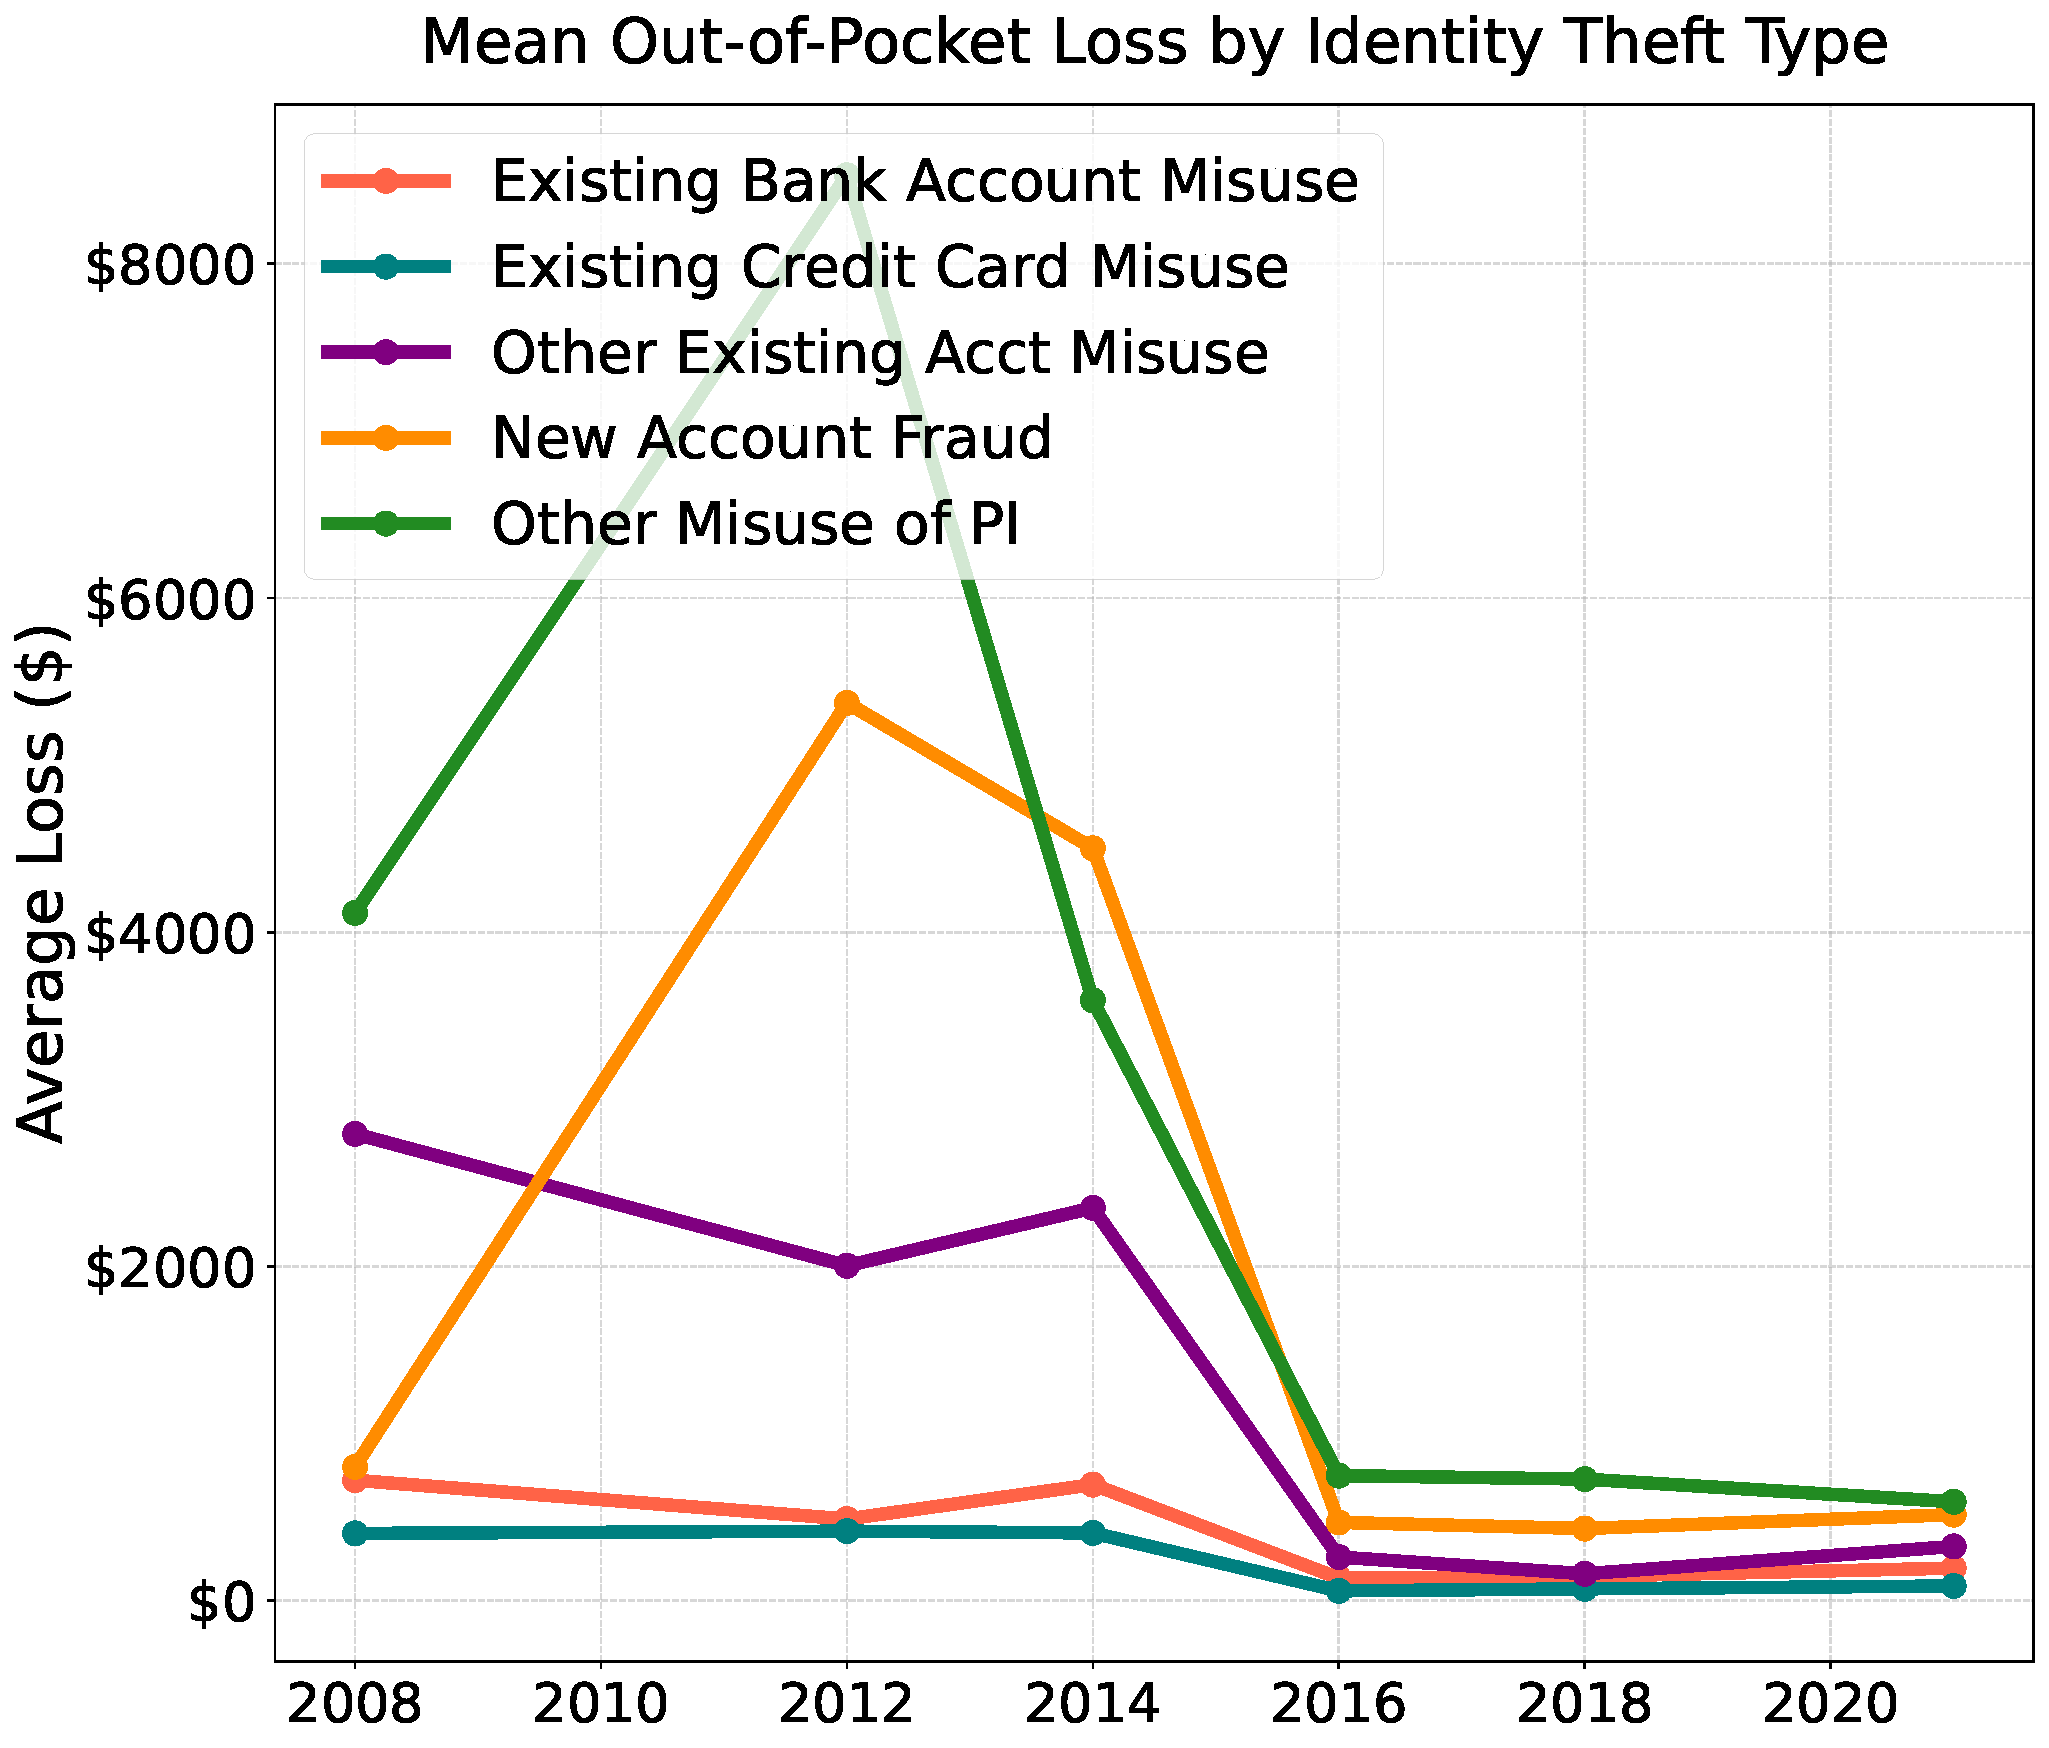
\includegraphics[width=0.48\textwidth]{figures/incident_trends/plot5_oop_loss_by_type.pdf}
    \caption{Mean Out-of-Pocket Loss by IDT Type (2008–2021).}
    \label{fig:oop_loss_comparison}
\end{wrapfigure}

Furthermore, a financial trend is evident in Figure \ref{fig:oop_loss_comparison}, which compares the average OOP losses adjusted to 2021 dollars, specifically for victims of different IDT types. It is worth noting that our OOP loss is less than direct loss values noted by BJS official reports \cite{HarrellThompson2024}, because we define OOP loss as the total amount of money stolen that was not recovered or reimbursed, so we include only costs that were not recoverable to the victim, rather than simply considering total amount stolen. 
%Both categories show a dramatic drop in average OOP loss between 2014 and 2016. 
Figure \ref{fig:oop_loss_comparison} shows that all categories show a drop and convergence between 2014 and 2016. This is the main driver behind the large drop in social cost observed in Table \ref{tab:social_costs_by_year}. We present two possible explanations for this trend. First, for the existing bank account misuse and existing credit card misuse OOP loss, we believe that the EMV transition played a dominant role as discussed above, because it reduced the most common type of high value, card-present fraud, and for the fraud that did occur, liability was clearer and banks had implemented faster detection systems, leading to more \$0 liability outcomes for consumers \cite{aba2018report}. Victims still reported ``credit card misuse'' because criminals pivoted to online, card-not-present fraud \cite{fed2018fraud}. This remote type of fraud is often more easily and quickly reimbursed by banks:  unlike in-person counterfeit fraud, where a dispute could be complex, as in a remote fraud case the victim is still in physical possession of their card, and bank systems can often use location data or IP addresses to quickly confirm that the transaction was fraudulent. This shift to a more easily reimbursable type of fraud meant the number of victims in our survey experiencing a direct, unrecoverable OOP loss fell dramatically, pulling the average loss for the entire group down. The EMV mandate applied to both credit and debit cards, the latter of which are the primary driver of bank account fraud losses according to a report by the American Bankers Association \cite{aba2018report}. While EMV chips directly impacted counterfeit card fraud, the concurrent drop for bank accounts represents this debit card protection as well as other broader improvements in banks' fraud detection systems \cite{aba2018report}.   



However, the fact that this drop is observed over all IDT categories, including those unrelated to the EMV mandate (although not nearly as dramatic), such as ``Other Misuse of PI'' and ``New Account Fraud,'' suggests that the structural changes to the ITS survey during 2016 may also have played a role. As mentioned earlier, in 2016 the survey underwent a sample redesign, where household sample sizes were increased by 41\%, and weights were recalibrated to reflect the 2010 Decennial Census \cite{Harrell2019Victims}. BJS mentions that these changes require caution when comparing 2016 estimates to previous waves \cite{Harrell2019Victims}. This survey shift likely explains the volatility seen in the ``Other Misuse of PI'' (which includes employment fraud or government benefit fraud), ``Other Existing Account Misuse'' (which includes utilities and telephone account misuse), and ``New Account Fraud'' categories, which were characterized by lower incidence rates but potentially very high value outlier losses. The surge in mean loss for these types in 2012 and 2014 is likely due to a few extreme outlier cases that affect the smaller sample mean. The stabilization after 2016 suggests that the improved, larger scale sampling better diluted the impact of high loss outliers that previously skewed averages.
%\com{Now that I'm looking at this data again, I feel the only one requiring some explanation is ``other existing acct misuse'', which did see a substantial drop, but not nearly as much as ``existing bank acct/CC misuse''. The other two fraud types did also decrease but comparatively minor. So yes, I think the shift in survey methodology likely did play a role but perhaps not as much as we/I originally thought...}
%\resp{Thanks Prof. Liu. I added some clarification above on (1) what other misuse of PI means (2) that we believe the EMV played a more dominant role over the survey restructuring, and (3) the other existing acct misuse}
